\label{sec:gnn_robust_and_faulty_modes}




\begin{figure}[t]
\centering

\begin{subfigure}{0.47\columnwidth}
    \centering
    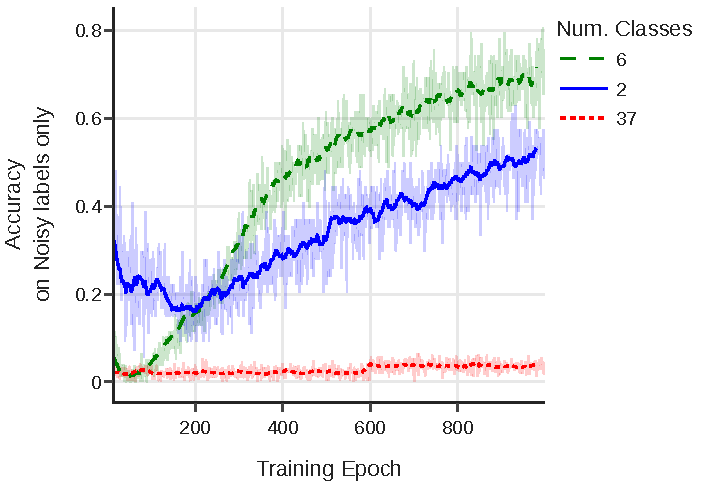
\includegraphics[width=\linewidth]{AISTATS/figures/fig3}
    \caption{}
    \label{fig:ppa_changing_number_of_classes}
\end{subfigure}\hspace{0.01\columnwidth}
\begin{subfigure}{0.47\columnwidth}
    \centering
    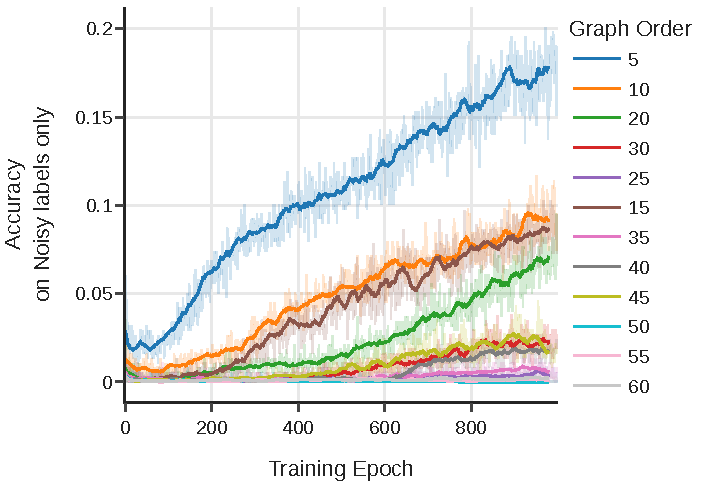
\includegraphics[width=\linewidth]{AISTATS/figures/fig2}
    \caption{}
    \label{fig:synthetic_data}
\end{subfigure}

\caption{
Training accuracy on noisy labels only. Effect of dataset properties:
(a) Fewer classes in PPA lead to faster overfitting on noise.
(b) Lower graph order leads to faster overfitting on noise.
}
\label{fig:various_figures}
\end{figure}



\begin{figure}[t]
\centering

\begin{subfigure}{0.48\columnwidth}
    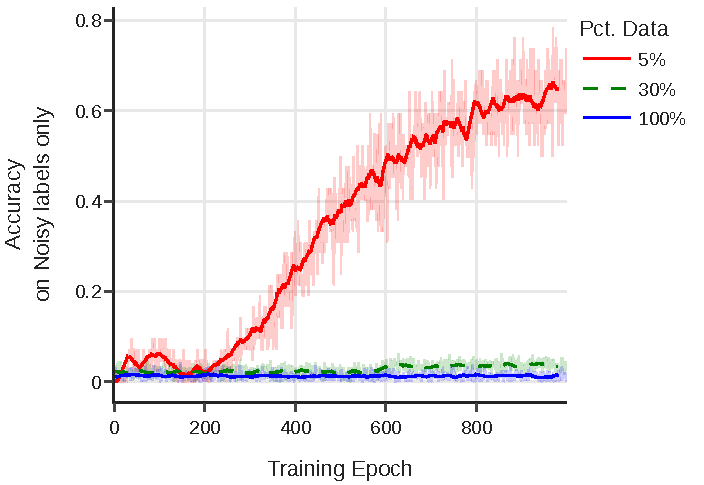
\includegraphics[width=\linewidth]{AISTATS/figures/fig4}
    \caption{}
    \label{fig:ppa_changing_number_of_smaples_of_class}
\end{subfigure}
\hfill
\begin{subfigure}{0.48\columnwidth}
    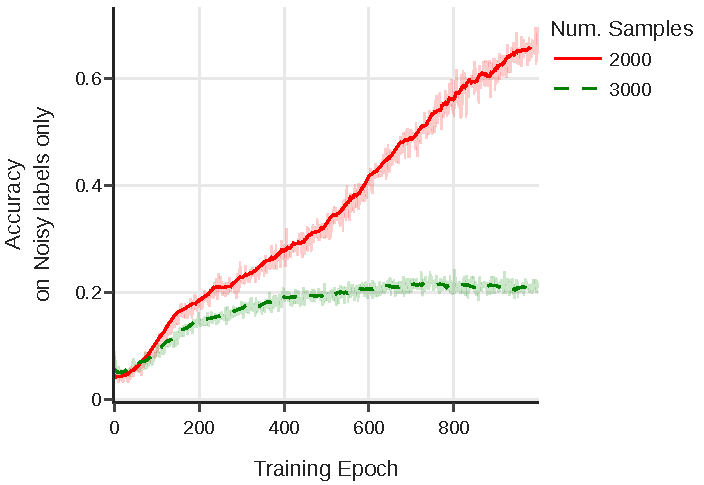
\includegraphics[width=\linewidth]{AISTATS/figures/fig5}
    \caption{}
    \label{fig:varying_samples_synthetic}
\end{subfigure}

\caption{Training accuracy on noisy labels only. Effect of dataset size: (a) Smaller fractions of the PPA dataset lead to stronger noise memorization. (b) Smaller synthetic datasets are also more prone to memorizing noise.}
\end{figure}


%
Before developing robust methods, we must understand when and why standard GNNs fail under label noise.
%
This section systematically investigates failure modes through controlled experiments, revealing that vulnerability depends on the relationship between model capacity and task complexity.
%
We begin by noting that GNNs exhibit surprising robustness in some settings.
% We study when and why a GNN applied to graph classification overfits noisy labels.
% Interestingly, GNNs exhibit a degree of inherent robustness. 
%
For instance, injecting noise into the full PPA  dataset ~\cite{PPA}, or large portions of it, does not significantly degrade model performance (see Fig.  \ref{fig:ppa_changing_number_of_classes}, \ref{fig:ppa_changing_number_of_smaples_of_class}, \ref{fig:noisy_pure_40_1}). 
%
We hypothesize that the observed robustness on PPA stems from the fact that the models may be under parameterized for the inherent difficulty of the PPA benchmark, on which state of the art methods struggle to achieve perfect accuracy\footnote{\url{https://paperswithcode.com/sota/graph-property-prediction-on-ogbg-ppa}}. 
%
This finding aligns with general findings that under parameterized models are often more robust to noise \cite{memorizenoise}.
%
Despite this, we show that GNNs nevertheless fail under certain conditions of label noise. 
% 
To examine this, we fix the model architecture and manipulate task complexity by (i) varying the number of classes as a proxy for over-parameterization, (ii) varying the average number of nodes in synthetic datasets, and (iii) varying the share of training data used. 
% 
We study the average training accuracy on noisy labels as a direct measure of how much the model fits noise. Higher accuracy on noisy samples indicates the model is memorizing them, while lower accuracy suggests that the model is not fitting the noise.

\textbf{GNN Robustness varying number of classes }
% 
We use 30\% of the PPA dataset and inject 20\% symmetric noise into this subset by randomly replacing labels with uniformly sampled incorrect classes.
% 
The model here and below, if not said otherwise, is a 5-layer Graph Isomorphism Network (GIN)~\cite{WL1} with 300 hidden units.
% 
Specifically, we create a sub-sampled PPA dataset with 2, 6, and the full 37 classes. 
% 
Intuitively, reducing the number of classes simplifies the classification task and reduces the effective dataset size, making the fixed model increasingly overparameterized relative to the task.
% 
Fig.~\ref{fig:ppa_changing_number_of_classes} shows the training accuracy on noisy samples across epochs. 
% 
For the full 37-class task, the GNN does not memorize noise and remains relatively robust. 
% 
However, when the number of classes is reduced to 6 and further to 2, the model increasingly fits the noisy labels. 
% 
Interestingly, the 2-class case exhibits slightly more robustness than the 6-class case due to the symmetric nature of the injected noise, since random flipping between two classes produces highly contrasting noisy samples.
% 

\textbf{GNNs are not robust on low-order graphs.}
% 
We generated synthetic datasets (see procedure in Appendix, Section \ref{appendix:details_synthetic_dataset_varying_nodes}) to study the effect of graph order (number of nodes). 
% 
As shown in Fig.~\ref{fig:synthetic_data}, GNNs become increasingly sensitive to noise as the graph order decreases. 
% 
Small graphs lack sufficient internal structure and aggregation capacity, making them vulnerable to treating noisy labels as signals.
% 
Conversely, larger graphs provide more nodes over which the model can average, diluting the influence of noisy samples.


\textbf{GNNs are not robust on small training sets.}  
% 
The size of a training set affects the robustness to noisy labels.
% 
For the PPA dataset, we keep all 37 classes, but subsample the number of training graphs per class. 
% 
As shown in Fig.~\ref{fig:ppa_changing_number_of_smaples_of_class}, reducing the number of training samples increases the likelihood of overfitting noise.
% 
A similar trend is observed for the synthetic datasets (with graph order 7 and 6 classes) under 35\% label noise, as shown in Fig.~\ref {fig:varying_samples_synthetic}.
% 
In both cases, models trained on smaller datasets have a higher tendency to memorize noisy samples due to insufficient clean data to learn generalizable patterns.




